\chapter{Types de contrôle}
\label{ch:controltypes}

\e
    \item Il existe 3 types de contrôle.
\ed

\section{Type 1}
\e
    \item \textbf{Lors d’un contrôle de type 1, chaque attaque doit être autorisée par le J-TAC/FAC(A).}
    \item Le contrôle de type 1 implique que le J-TAC/FAC(A) aie le contact visuel sur la cible, ainsi que le contact visuel sur l’appareil au moment de l’attaque.
    \item Ce type de contrôle est utilisé lorsque le risque de tir ami est considéré élevé.
    \item Le J-TAC/FAC(A) donnera l’autorisation de tir (“cleared hot”) au dernier moment, lorsqu’il sera certain que l’appareil engage la bonne cible.
    \item Un contrôle de type 1 se déroule comme suit:
    \ee
        \item Acquisition visuelle de la cible par le J-TAC/FAC(A)
        \item Gameplan/CAS brief
        \item Readback lignes 4, 6 et 8
        \item Annonce “IP INBOUND”
        \item Annonce “IN”
        \item Le J-TAC/FAC(A) acquiert visuellement l’appareil qui attaque
        \item Le J-TAC/FAC(A) annonce “CLEARED HOT”, “CONTINUE DRY” ou “ABORT”
    \ed
\ed

\section{Type 2}
\e
    \item \textbf{Lors d’un contrôle de type 2, chaque attaque doit être autorisée par le J-TAC/FAC(A).}
    \item Le contrôle de type 2 est utilisé lorsque le J-TAC/FAC(A) lorsque le J-TAC/FAC(A) ne peut pas obtenir le visuel, soit sur la cible, soit sur l’appareil au moment du largage de la munition.
    \item Un contrôle de type 2 se déroule comme suit:
    \ee
        \item Acquisition de la cible par le J-TAC/FAC(A), visuellement ou par d’autres moyens
        \item Gameplan/CAS brief
        \item Readback lignes 4, 6 et 8
        \item Annonce “IP INBOUND”
        \item Annonce “IN” + cap d’attaque ou cap depuis la cible (ex: “IN 340”, ou “IN depuis le sud”)
        \item Le J-TAC/FAC(A) acquiert visuellement l’appareil qui attaque
        \item Le J-TAC/FAC(A) annonce “CLEARED HOT”, “CONTINUE DRY” ou “ABORT”
    \ed
\ed

\section{Type 3}
\e
    \item Le contrôle de type 3 est utilisé lorsque le J-TAC/FAC(A) requiert \textbf{plusieurs attaques} en un seul \textbf{engagement}.
    \item Un contrôle de type 3 se déroule comme suit:
    \ee
        \item Acquisition de la cible par le J-TAC/FAC(A), visuellement ou par d’autres moyens
        \item Gameplan/CAS brief
        \item Readback lignes 4, 6 et 8
        \item Annonce “IP INBOUND”
        \item Annonce “IN”
        \item Le J-TAC/FAC(A) acquiert visuellement l’appareil qui attaque
        \item Le J-TAC/FAC(A) annonce “CLEARED TO ENGAGE” ou “CONTINUE DRY”
        \item Avant le tir de la première munition, l’appareil qui attaque annonce “COMMENCING ENGAGEMENT”
        \item Une fois l’engagement terminé, l’appareil annonce “ENGAGEMENT COMPLETE”
    \ed
\ed

\section{Méthodes d’attaque}
\e
    \item
    Il existe deux méthodes d’attaque: “Bomb on target”, et “Bomb on coordinates”. Bomb on target implique l’acquisition de la cible par l’appareil en attaque, et le largage de munition sur cette dernière, alors que le Bomb on coordinates implique le largage de munitions intelligentes sur des coordonnées, sans pour autant devoir “voir” la cible.
    \item En Kamov, on utilisera systématiquement le BOT.
\ed

\section{Résumé des types de contrôle et des méthodes d’attaque}
\e
    \item
    Extrait du \jp:
\ed
\makebox[\textwidth]{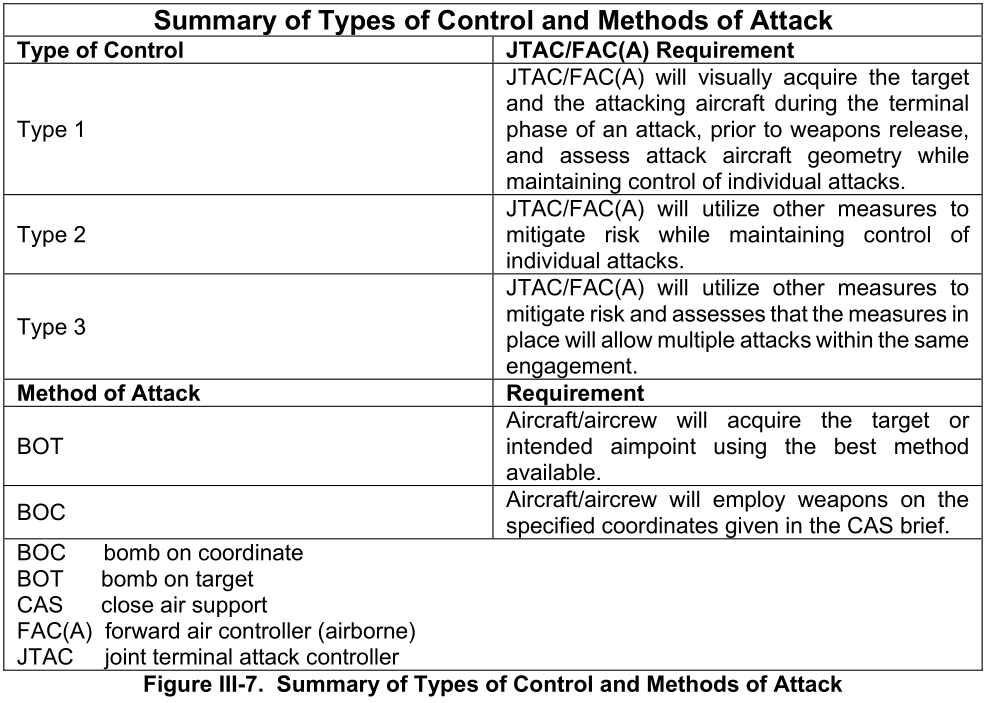
\includegraphics[width=0.9\paperwidth]{controltypes.png}}
% TODO missing figure ref



